\section{First Order Differential Equations}
In this section, we deal with differential equations of the form
\[ \dv{x}{t} = f(x, t) \]
There is no general way to solve these equations, but there are certain types that we can solve. We have already explored separable first order differential equations in Section \ref{separablesection}, and now we will focus on first order linear equations.
\subsection{First Order Linear Differential Equations}
A \bf{first order linear differential equation} is any first order differential equation that can be written in the form
\[ \dv{x}{t} + p(t)x = g(t) \]
We can also write it as
\[ P(t)\dv{x}{t} + Q(t)x = G(t)\]
which will sometimes be more convenient. Of course, it is simple to convert between these two forms as long as $P(t)\neq 0$. \par
For now, we will stick with the first form. Suppose we have a differential equation of that form that is defined on some domain $D$. We will multiply both sides of the equation by some mystery function $\mu(t)$ (we will come back and explore how to figure out what this $\mu(t)$ is) that is also defined on $D$ to obtain
\[ \mu(t) \dv{x}{t} + \mu(t)p(t)x = \mu(t)g(t) \]
You may notice that the left hand side of this equation looks somewhat like a product rule. If we make the proposition that $\mu '(t) = \mu(t)p(t)$, we can write 
\[ \mu(t)\dv{x}{t} + \mu(t)p(t)x = \dv{t} \pqty{\mu(t)x(t)} \]
allowing us to write our full equation as
\[ \dv{t} \pqty{\mu(t)x(t)} = \mu(t)g(t) \]
Integrating both sides with respect to $t$, we obtain
\[ \mu(t)x(t) = \int \mu(t)g(t)\dd t + C\]
and dividing by $\mu(t)$, provided that $\mu(t)\neq 0$, we get
\[ x(t) = \frac{1}{\mu(t)}\int \mu(t)g(t)\dd t + \frac{1}{\mu(t)}C \]
Now, what is $\mu(t)$? Recall the earlier assumption that we made:
\[ \dv{\mu(t)}{t} = \mu(t)p(t) \]
This is a separable equation that can be solved.
\begin{align*}
    \frac{1}{\mu(t)}\dv{\mu(t)}{t} &= p(t) \\
    \int \frac{1}{\mu(t)}\dv{\mu(t)}{t}\dd t &= \int p(t)\dd t \\
    \ln\abs{\mu(t)} &= \int p(t)\dd t
\end{align*}
Which gives us
\[ \mu(t) = \pm e^{\int p(t)\dd t} \]
Because we are choosing $\mu(t)$ ourselves, we can just choose the positive solution and discard the negative one. Additionally, we will sometimes write 
\[ \mu(t) = \exp \int p(t)\dd t\]
Where $\exp$ is the function $\exp(x) = e^x$, simply to make it easier to read. \par
We will exclude the $+C$ here as it is included later in the calculation. Plugging this back into our equation for $x(t)$, we obtain
\[ x(t) = e^{-\int p(t)\dd t}\pqty{\int g(t) e^{\int p(t)\dd t}\dd t + C}\]
This formula is clunky and can be difficult to remember. Instead of attempting this, simply go through the process of finding $\mu(t)$ and reversing the product rule each time--it is much easier.
\begin{example}
    Use the method of integrating factors to solve the initial value problem
    \[ t\dv{x}{t} + 2x = 4t^2 \]
    with $x(1) = 2$. \par
    \bf{Solution:} First, we will get our equation in standard form. Dividing both sides by $t$, we get (with the added restriction that $t\neq 0$), 
    \[ \dv{x}{t} + \frac{2}{t}x = 4t \]
    With this, our integrating factor $\mu(t)$ is
    \[ \mu(t) = e^{\int 2t^{-1}\dd t} = e^{2\ln|t|} = |t^2| = t^2\] 
    Multiplying both sides by $\mu(t)$, we get
    \[ t^2\dv{x}{t} + 2tx = 4t^3 \]
    recognizing the inverse product rule, we can rewrite this as
    \[ \dv{t} \pqty{t^2x} = 4t^3\]
    Which becomes
    \begin{align*}
        t^2x &= t^4 + C \\
        x(t) &= t^2 + \frac{C}{t^2}
    \end{align*}
    With the initial condition $x(1)=2$, we find
    \[ x(1) = 2 = 1 + C \quad \implies \quad C = 1\]
    and
    \[ x(t) = t^2 + t^{-2}\] 
    Recall from the definition of a solution to a differential equation, this is only valid on the region where $t>0$. It turns out that the general solution on $t<0$ is identical in this case, but that does not tell us anything about the particular solution. \par
    This becomes paricularly important to pay attention to in cases where the solution does not have a discontinuity where the original differential equation does. For example, if our initial condition was instead $x(1) = 1$, we would get $C=0$ and the particular solution would be $x(t) = t^2$. However, despite the lack of a discontinuity at $t=0$ in our solution, this is still only valid for $t>0$.
\end{example}
\begin{example}
    Use the method of integrating factors to solve the initial value problem 
    \[ 2\dv{y}{x} + xy = 2 \]
    with $y(0) = 1$. \par
    \bf{Solution:} First, get the equation into standard form.
    \[ \dv{y}{x} + \frac{x}{2}y = 2\]
    This does not introduce any domain restrictions. Then, compute $\mu(x)$.
    \begin{align*}
        \mu(x) &= e^{\int x/2 \dd x} \\
        &= e^{x^2/4}
    \end{align*}
    Multiplying both sides by $\mu(x)$
    \begin{align*}
        e^{x^2/4}\dv{y}{x} + e^{x^2/4}\frac{x}{2}y &= 2e^{x^2/4} \\
        \dv{x}\pqty{ye^{x^2/4}} &= 2e^{x^2/4} \\
        &= ye^{x^2/4} \\
        ye^{x^2/4} &= 2\int e^{x^2/4}\dd x + C
    \end{align*}
    This integral is not able to be evaluated in terms of elementary functions, so we will just leave it unevaluated. Instead, we can make it a definite integral to give us a single function. We will make the lower bound of our integral the $x$ value of our initial condition, which in this case is $x=0$. Therefore, we obtain
    \begin{align*}
        y(x) = 2e^{-x^2/4}\int_0^x e^{s^2/4}\dd s + C 
    \end{align*}
    where $s$ is a dummy variable, so that we do not have $t$ representing two different things. Plugging in for our initial condition, we get
    \begin{align*}
        y(0) = 1 = 2e^0 \int_0^0 e^{s^2/4}\dd s + C \quad \implies \quad C = 1
    \end{align*}
    So we get
    \[ y(x) = 2e^{-x^2/4}\int_0^x e^{s^2/4}\dd s + 1 \]
\end{example}
It is perfectly acceptable to leave a solution in terms of an integral, since even functions that have no elementary antiderivative can have their integrals approximated to high levels of accuracy with computers. \par
Sometimes, differential equations of the form 
\[ \dv{y}{x} = f(x,y) \]
have a constant solution $y=y_0$. These are quite easy to spot because they occur when $f(x, y_0) = 0$ for all $x$ on the interval of the solution.
\begin{example}
    Find the constant solutions of the differential equation 
    \[ \dv{y}{x} = \cos (x)\pqty{ e^{x/4}}(y)(y-2)(y+5) \]
    \bf{Solution:} Because of the three factors $y$, $y-2$, and $y+5$ in $\dv{y}{x}$, we have $\dv{y}{x}=0$ whenever $y=0$, $y=2$ and $y=-5$. These are the constant solutions to the differential equation, and they are valid on the domain $(-\infty, \infty)$, because there are no discontinuities in the expression for $\dv{y}{x}$.
\end{example} 
\subsection{Modeling with First-Order Differential Equations}
In this section, we explore a couple of real world examples that can be modeled with differential equations.
\begin{example}
    Imagine a large tank with a volume $V$ where liquid is both entering and exiting the tank at a constant rate of $R$ liters per minute. The liquid entering the tank has a constant concentration of $C_I$ pounds per gallon of a substance (this may be salt, pollutants, etc.), and the liquid entering the tank mixes with the liquid in the tank instantly. At $t=0$, the amount of substance in the tank is $Q_0$. Find an expression for the amount of substance in the lake as a function of time. \par
    \bf{Solution:} The rate of change of concentration in the tank is given by
    \[ \dv{Q}{t} = (\text{concentration in})(\text{volume in}) - (\text{concentration out})(\text{volume out})\]
    The concentration in is $C_I$, the volume in and out is $R$, and the concentration out is given by $C(t)$, a function that describes the concentration of substance at any particular time $t$. This gives us
    \[ \dv{Q(t)}{t} = RC_I - RC(t)\]
    Since the amount of substance is equal to the concentration times the volume--$Q=CV$--we can rewrite to obtain
    \[ \dv{Q(t)}{t} = RC_I - \frac{R}{V}Q(t)\] 
    Which is a first order linear equation. In standard form, it is
    \[ \dv{Q}{t} + \frac{R}{V}Q(t) = RC_I\]
    The integrating factor is $\mu(t) = e^{\int R/V\dd t} = e^{tR/V}$, and we find
    \[ e^{tR/V}\dv{Q}{t} + \frac{R}{V}e^{tR/V}Q(t) = e^{tR/V}RC_I \]
    Which, with an inverse product rule, becomes
    \begin{align*}
        \dv{t}\pqty{Q(t)e^{tR/V}} &= e^{Rt}RC_I \\
        Q(t) &= e^{-tR/V}\int e^{tR/V}RC_I\dd t + Ce^{-tR/V}\\
        &= \frac{V}{R}e^{-tR/V}e^{tR/V}RC_I +Ce^{-tR/V}\\
        &= VC_I + Ce^{-tR/V}
    \end{align*}
    With the initial condition $Q(0)=Q_0$, we find
    \[ Q(0) = Q_0 = VC_I+C \]
    which tells us $C = Q_0 - VC_I$. Thus, we obtain
    \[ Q(t) = VC_I + \pqty{Q_0-VC_I}e^{-tR/V}\]
    As $t\to\infty$, the exponential decay term will dissipate and we are left with
    \[ \lim_{t\to\infty}Q(t) = VC_I \]
    which tells us that the final concentration is equal to the concentration of the incoming water. This makes sense, as eventually the incoming water will by fully mixed with the water in the tank. 
\end{example}
% \begin{example}
%     Imagine a large tank with an initial volume of $V_0$ where liquid is both entering and exiting the tank at a constant rate of $R_I$ and $R_O$ liters per minute respectively. The liquid entering the tank has a constant concentration of $C_I$ pounds per gallon of a substance (this may be salt, pollutants, etc.), and the liquid entering the tank mixes with the liquid in the tank instantly. \par
%     At $t=0$, the amount of substance in the tank is $Q_0$. Find a function describing the amount of substance in the tank at any time $t$. \par
%     The rate of change of concentration in the tank is given by
%     \[ \dv{Q}{t} = (\text{concentration in})(\text{volume in}) - (\text{concentration out})(\text{volume out})\]
%     The concentration in is $C_I$, the volume in is $R_I$, the volume out is $R_O$, and the concentration out is given by $C(t)$, a function that describes the concentration of substance at any particular time $t$. This gives us
%     \[ \dv{Q(t)}{t} = R_IC_I - R_OC(t)\]
%     Since the amount of substance is equal to the concentration times the volume--$Q(t)=C(t)V(t)$--we can rewrite to obtain
%     \[ \dv{Q(t)}{t} = R_IC_I - \frac{R_O}{V(t)}Q(t)\] 
%     The volume as a function of time is given by 
%     \[ \text{Volume} = \text{Initial Volume} + (\text{Rate in})(\text{time}) - (\text{Rate out})(\text{time}) \]
%     which is, in equation form,
%     \[ V(t) = V_0 + R_It - R_Ot \]
%     Which we can plug back into the expression for $\dv{Q}{t}$ to find
%     \[ \dv{Q(t)}{t} = R_IC_I - \frac{R_O}{V_0+(R_I-R_O)t}Q(t) \]
%     This is a first order linear equation. In standard form, it is
%     \[ \dv{Q}{t} + \frac{R_O}{V_0+(R_I-R_O)t}Q(t) = R_IC_I\]
%     The integrating factor is 
%     \begin{align*}
%         \mu(t) &= \exp \pqty{\int \frac{R_O}{V_0 + (R_I-R_O)t}\dd t} \\
%         &= \exp \pqty{\frac{R_O}{R_I-R_O}\ln\abs{V_0+(R_I-R_O)t}} \\
%         &= \abs{\bqty{V_0+(R_I-R_O)t}^{R_0/(R_I-R_O)}}
%     \end{align*}
%     As long as the volume is positive $V_0 + (R_I-R_O)t$ will also be positive, and we can remove the absolute value bars, giving us
%     \[ \mu(t) = \pqty{V_0+(R_I-R_O)t}^{R_O/(R_I-R_O)}\]
%     Define the difference in flow rate as $\Delta R = R_O - R_I$, which allows us to write
%     \[ \mu(t) = \pqty{V_0 - t\Delta R}^{-R_O/\Delta R}\]
%     Now, multiplying $\mu(t)$ into both sides of our differential equation, we find
%     \[ \pqty{V_0 - t\Delta R}^{-R_O/\Delta R}\dv{Q}{t} + \pqty{V_0 - t\Delta R}^{-R_O/\Delta R}\frac{R_O}{V_O-t\Delta R}Q = \pqty{V_0 - t\Delta R}^{-R_O/\Delta R}R_IQ_I\]
%     Which, with an inverse product rule, becomes
%     \begin{align*}
%         \dv{t}\pqty{Q(t)\pqty{V_0 - t\Delta R}^{-R_O/\Delta R}} &= \pqty{V_0 - t\Delta R}^{-R_O/\Delta R}R_IC_I
%     \end{align*}
%     And then
%     \begin{align*}
%         Q(t) &= (V_0-t\Delta R)^{R_O/\Delta R}\int R_IC_I(V_0-t\Delta R)^{-R_O/R}\dd t + (V_0-t\Delta R)^{R_O/\Delta R}C\\
%         &= \frac{R_IC_I}{\Delta R}\frac{\Delta R}{R_O}(V_0-t\Delta R)^{R_O/\Delta R}(V_0-t\Delta R)^{-R_O/\Delta R + 1} + (V_0-t\Delta R)^{R_O/\Delta R}C\\
%         &= \frac{R_IC_I}{R_O} (V_0-t\Delta R) + (V_0-t\Delta R)^{R_O/\Delta R}C
%     \end{align*}
%     With the initial condition $Q(0)=Q_0$, we find
%     \[ Q(0) = Q_0 = \frac{V_0R_IC_I}{R_O}+(V_0-t\Delta R)^{R_O/\Delta R}C \]
%     which tells us 
%     \[ C = \frac{Q_0 - \frac{V_0R_IC_I}{R_O}}{V_0^{R_O/\Delta R}} = \frac{Q_0}{V_0^{R_O/\Delta R}} - \frac{V_0^{1-R_O/\Delta R}R_IC_I}{R_O}\]
%     and
%     \[ Q(t) = \frac{R_IC_I}{R_O} (V_0-t\Delta R) + (V_0-t\Delta R)^{R_O/\Delta R}\pqty{\frac{Q_0}{V_0^{R_O/\Delta R}} - \frac{V_0^{1-R_O/\Delta R}R_IC_I}{R_O}}\]
%     I don't think any of us really want to do much analysis on this result, so we won't
% \end{example}
\begin{example}
    Consider the previous example, but the concentration of chemical in the incoming water is given by a function of time $C_I(t)$ instead of being constant at $C_I$. Find an expression for the amount of substance in the tank as a function of time. \par
    \bf{Solution:} In this case, the governing differential equation becomes 
    \[ \dv{Q}{t} = RC_I(t) - \frac{R}{V}Q(t) \]
    Which is a linear first order differential equation. Our integrating factor is $\mu(t) = e^{Rt/V}$, which gives us
    \begin{align*}
        \dv{t}\pqty{e^{Rt/V}Q(t)} &= RC_I(t)e^{Rt/V} \\
        Q(t) &= Re^{-Rt/V}\int C_I(t)e^{Rt/V}\dd t
    \end{align*}
    If, for example, the concentration is given by $C_I(t) = \alpha + \beta\sin(t)$, we get
    \begin{align*}
        Q(t) &= Re^{-Rt/V}\int \pqty{\alpha e^{Rt/V} + \beta e^{Rt/V}\sin(t)}\dd t + ce^{-Rt/V} \\
        &= \alpha V + \frac{\beta RV (R\sin t - V\cos t)}{V^2+R^2} + ce^{-Rt/V}
    \end{align*}
    If $Q(0) = Q_0$, then
    \[ Q(0) = Q_0 = \alpha V - \frac{\beta RV^2}{V^2+R^2} + c \]
    which tells us
    \[ Q(t) = \alpha V + \frac{\beta RV (R\sin t - V\cos t)}{V^2+R^2} + \pqty{Q_0 + \frac{\beta RV^2}{V^2+R^2}- \alpha V} e^{-Rt/V}\]
    If we plug in some values for our constants and plot it, we get a graph that looks something like this:
    \begin{figure}[h!]
        \centering
        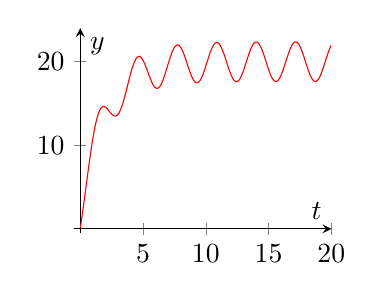
\begin{tikzpicture}
            \begin{axis}[width=0.4\textwidth, axis lines=middle, xlabel=$t$, ylabel=$y$, xmin=-.5, ymin=-.5, ymax=24, xmax=20]
                \addplot[color=red,domain=0:20,samples=200]{20 - 2.3 * cos (2 * x * 180 / pi) + 0.58 * sin (2 * x * 180 / pi ) - 17.64 * e^(-0.5 * x)};
            \end{axis}
        \end{tikzpicture}
    \end{figure}
    This shows the concentration of pollutants in the tank increasing from the initial value up to the concentration of the intake water, and then oscillating as the concentration of the intake changes.
\end{example}
\begin{example}
    Suppose that a sum of money $S_0$ is deposited in a bank that pays interest continuously at an annual rate $r$. Additionally suppose that the customer adds money to the bank account at a constant rate of $k$ dollars per year. Find an expression for the amount of money in the bank account as a function of time. \par
    \bf{Solution:} The governing differential equation for this scenario is 
    \[ \dv{S}{t} = rS + k \]
    with the initial condition $S(0) = S_0$. The solution to this equation can be easily found by the method of separation of variables:
    \begin{align*}
        \int \frac{1}{rS+k}\dv{S}{t}\dd t &= \int \dd t \\
        \frac{1}{r}\ln \abs{rS+k} &= t + C \\
        S(t) = Ce^{rt}-\frac{k}{r}
    \end{align*}
    The initial condition is $S(0) = S_0 = C-k/r$ so we get $C = S_0 + k/r$, and
    \[ S(t) = S_0e^{rt} + \frac{k}{r}\pqty{e^{rt}-1}\]
    The first term accounts for the exponential growth of the initial sum and the second term accounts for the additional money added over time, as well as its growth.
\end{example}
\subsection{Differences Between Linear and Nonlinear Differential Equations}
\subsubsection{Existence and Uniqueness of Solutions}
In all of the previous examples, we have seen differential equations with one and exactly one solution. This leads to the question of when we might find differential equations with more than one solution, or perhaps no solution at all. For first order linear differential equations, this question is answered by the \bf{existence and uniqueness} theorem.
\begin{theorem}[Existence and Uniqueness of Solutions to First Order Linear Differential Equations]
    Suppose $p$ and $g$ are continuous on some interval $I = (\alpha, \beta)$, that contains the point $t=t_0$. Then, there exists a unique function $x=\varphi(t)$ that satisfies the differential equation
    \[ \dv{x}{t} + p(t)x = g(t) \]
    for all $t\in I$, and for which $x(t_0) = x_0$.
\end{theorem}
The proof of this theorem is simple, and naturally follows from our derivation of the general solution to a first order linear differential equation. Critically, this tells us that solutions to first order linear differential equations on an interval are unique--provided that there are no discontinuities in the equation. \par
For nonlinear first order equations, the statement becomes a little more complicated.
\begin{theorem}[Existence and Uniqueness of Solutions to General First Order Differential Equations] 
    \label{exuniq}
    Let the functions $f$ and $\partial f / \partial x$ be continuous in some rectangle $R = [t_0 - a, t_0 + a] \times [x_0 - b, x_0 + b]$ surrounding $(x_0, t_0)$. Then, there is a unique solution to the initial value problem 
    \[ \dv{x}{t} = f(x,t), \quad x(t_0) = x_0 \] 
    on some interval $[t_0 - h, t_0 + h]$ with $0 < h < a$.
\end{theorem}
If we only had the continuity of $f$ and not the continuity of $\partial f/\partial x$, then we can guarantee the existence of a solution, but not its uniqueness. \par 
One important result of this theorem is that the graphs of two solutions to a differential equation (that satisfies existence and uniqueness) cannot cross over each other. If there are two different functions $\varphi(t)$ and $\psi(t)$ that intersect at $(t_0, \varphi(t_0)) = (t_0, \psi(t_0))$ and satisfy the differential equation, then that means we have two nonunique solutions to the same initial value problem, which is not possible.
\begin{example}
    Find the interval for which the initial value problem
    \[ x\dv{y}{x} + 2y = 4x^2 \quad y(1) = 2\]
    Has a unique solution. Do the same for when the initial condition is changed to $y(-1) = 2$. \par
    \bf{Solution:} First, rewrite the differential equation in standard form to obtain
    \[ \dv{y}{x} + \frac{2}{x} y = 4x \]
    This gives us $p(x) = 2x^{-1}$ and $g(x) = 4x$. $g$ is continuous everywhere, but $p$ has a discontinuity at $x=0$. Therefore, there are two intervals of continuity for $p$: $(-\infty, 0)$ and $(0, \infty)$. \par
    For the initial condition $y(1)=2$, it clearly lies on the interval $x\in (0, \infty)$, so that is the interval of our solution. For the other condition, it lies on $x\in(-\infty, 0)$, so that is the interval of our solution.
\end{example}
\begin{example}
    Use Theorem \ref{exuniq} to analyze the interval of existence and uniqueness of solutions to the initial value problem
    \[ \dv{y}{x} = \frac{3x^2+4x+2}{2(y-1)}\] 
    for both $y(0)=-1$ and $y(0)=1$. \par
    \bf{Solution:} Recall that Theorem \ref{exuniq} states that a differential equation of the form $\dd y/\dd x = f(x,y)$ is guaranteed a unique solution on a connected interval where $f(x,y)$ and $\pdv{y} f(x,y)$ are continuous. Computing $\partial f/\partial y$, we find
    \[ \pdv{f}{y} = \frac{-(3x^2+4x+2)}{2(y-1)^2} \]
    Both $f$ and $\partial f/\partial y$ are uniformly continuous except on the line $y=1$. Because there is a neighborhood around the point $(0, -1)$ where $f$ and $\partial f/\partial y$ are continuous, there exists some nonempty interval $[a,b]$ around $x=0$ where there is a unique solution to the differential equation. We are not able to tell exactly what this interval is without attempting to solve the equation, however. \par
    For the second initial condition, there is no neighborhood around $(0, 1)$ where $f$ or $\partial f/\partial y$ are continuous, so we cannot guarantee the existence or uniqueness of a solution on that interval. \par
    It turns out in this case that two solutions exists that satisfy $y(0)=1$, but clearly these solutions are not unique. We are also unable to guarantee the existence of these solutions without attempting to solve the problem. 
\end{example}
\begin{example}
    Apply Theorem \ref{exuniq} to the initial value problem
    \[ \dv{y}{x} = y^{1/3} \quad y(0)=0\]
    and solve it. \par
    \bf{Solution:} The function $f(x,y) = y^{1/3}$ is continuous everywhere, but $\partial f/\partial y = y^{-2/3}/3$ is discontinuous at $y=0$. Hence for the initial condition $y(0)=0$, we can guarantee the existence, but not the uniqueness, of a solution on some interval $[a,b]$ around $x=0$. \par
    We can go about solving this equation as we would with any other separable equation. 
    \begin{align*}
        \int \frac{1}{y^{1/3}}\dv{y}{x}\dd x &= \int \dd x \\
        \intertext{Note that some issues will arise with the fact that $y=0$ must be included in the domain of the solution, which causes $y^{-1/3}$ to be undefined. We will simply ignore this and solve normally, returning later to make sure that the solution is still valid for $y=0$.}
        \frac{3}{2}y^{2/3} &= x+C \\
        y(x) &= \pm \pqty{\frac{2}{3}x + C}^{3/2}
    \end{align*}
    The initial condition $y(0)=0$ is satisfied by a few functions: $\phi_1 (x) = \pqty{\frac{2}{3}x}^{3/2}$, $\phi_2 (x) = -\pqty{\frac{2}{3}x}^{3/2}$, and the constant solution $\psi (x)=0$. The domains of the first two solutions are $[0, \infty)$ and the domain of the final solution is $\RR$. In fact, we will have infinitely many solutions. Notice that the function
    \[ \chi_{t_0}(x) = \begin{cases}
        0 & -\infty < t < t_0 \\
        \pm \pqty{\frac{2}{3}(x-t_0)}^{3/2} & t_0 \leq t < \infty
    \end{cases}\]
    satisfies the initial value problem for any $t_0 \geq 0$.
\end{example}
\subsubsection{Interval of Existence}
The above example illustrates an important consequence of Theorem $\ref{exuniq}$. While the interval of existence of a solution to the first order linear equation $y' + p(t)y = g(t)$ is easy to determine by analyzing the continuity of $p$ and $g$, the case where we have $y' = f(t, y)$ is more complicated. As we saw in the previous example, the points of discontinuity or non-existence of a solution $y = \phi(t)$ may have no simple relationship to the points of discontinuity of $f$. 
\begin{example}
    Solve the initial value problem 
    \[ \dv{y}{x} = y^2 \quad y(0)=1\]
    and determine the interval for which the solution exists. \par
    \bf{Solution:} Theorem $\ref{exuniq}$ guarantees a unique solution on all of $\RR$ because $y^2$ and $\pdv{y}y^2 = 2y$ are both continuous everywhere. We can then use the method of separation of variables to solve it.
    \begin{align*}
        \int \frac{1}{y^2}\dv{y}{t}\dd t &= \int \dd t \\
        -\frac{1}{y} &= t + C \\
        y &= \frac{-1}{t+C}
    \end{align*}
    With the initial condition $y(0)=1$, we find $1 = -1/C$ which tells us $C=-1$ and that
    \[ y(t) = \frac{1}{1-t} \]
    This has a discontinuity at $t=1$, so the two regions of continuity are $(-\infty, 1)$ and $(1, \infty)$. Because the initial condition is at $t=0$, our solution is defined on the left interval and we obtain
    \[ y(t) = \frac{1}{1-t} \qquad y < 1 \]
    If we instead had an initial condition $y(0) = y_0$ with $y_0 \neq 0$, we would get $C = -1/y_0$ and a general solution given by
    \[ y(t) = \frac{y_0}{1-y_0t}\]
    This gives us two regions of continuty: $(-\infty, 1/y_0)$ and $(1/y_0, \infty)$. If $y_0$ is positive, $t=0$ (and thus the solution) lies in the right region. If $y_0$ is negative, the solution lies in the left region. 
\end{example}
This illustrates another critical feature of initial value problems for nonlinear equations: the locations of discontinuities and the interval of existence of the solution(s) may depend on the initial condition. 
\subsubsection{General Solutions}
Another difference between linear and nonlinear equations concerns the idea of a general solution. For linear equations, we found that we could represent all possible solutions with one arbitrary constant. This may not be the case for nonlinear equations. \par
For instance, in the previous example, we found a ``general solution'' given by 
\[ y(1) = \frac{-1}{t+C} \]
The arbitrary constant present in this, however, fails to encompass all solutions because the constant solution $y=0$ also solves the equation, but cannot be achieved with any value of $C$.
\subsubsection{Implicit Solutions}
Recall that we are always able to find an explicit formula for the solution to a first order linear differential equation with
\[ y(t) = \frac{1}{\mu(t)}\pqty{\int \mu(t)g(t)\dd t + C}\]
Thus the value of $y(t)$ could be found for any $t$ simply by plugging in. For nonlinear equations, this is not always the case. Oftentimes the best we can hope for is an implicit solution of the form
\[ F(t, y) = 0 \]
that is satisfied by a function $y = \phi(t)$ such that $F(t, \phi(t)) = 0$ on the domain of $\phi$. We call the above equation an \bf{integral} of the differential equation. Its graph is called an \bf{integral curve}, or a family of integral curves. \par
In cases where $F(t,y)$ cannot be turned into an explicit solution, we must solve for $y$ separately with each value of $t$. We can then plot some of these $(t,y)$ pairs in order to get a rough sketch of what a solution looks like. Alternatively, computer tools can plot the graph described by $F(t,y)=0$, which we can analyze. \par
We will also frequently encounter first order equations where not even an implicit solution can be found. These must be analyzed through approximations, and can be very difficult to work with. Tools such as direction fields or numerical methods prove particularly beneficial with these equations.
\subsection{Bernoulli Equations}
Sometimes it is possible to solve a nonlinear equation by making a change in the dependend variable that converts a nonlinear equation into a linear equation. One such equation has the form
\[ \dv{y}{t} + p(t)y = q(t)y^n \]
and is known as a Bernoulli equation. If we make the substitution $u = y^{1-n}$, we can rearrange to find $y = u^{1/(1-n)}$. \par
From this, use the chain rule to obtain
\[ \dv{y}{t} = \dv{y}{u}\dv{u}{t} = \bqty{\frac{1}{1-n}u^{1/(1-n)-1}}\dv{u}{t} \]
or
\[ \dv{y}{t} = \bqty{\frac{1}{1-n}u^{n/(1-n)}}\dv{u}{t} \] 
Substituting this in, we obtain
\[ \bqty{\frac{1}{1-n}u^{n/(1-n)}}\dv{u}{t} + p(t)u^{1/(1-n)} = q(t)u^{n/(1-n)}\]
which can be simplified to
\[ \dv{u}{t} + (1-n)p(t)u = (1-n)q(t)\]
Which is a linear equation with the dependent variable $u$ that can be solved.
\begin{example}
    Using the method illustrated above, find the general solution to the equation
    \[ \dv{y}{t} = \epsilon y - \sigma y^3\]
    with $\epsilon, \sigma >0$. \par
    \bf{Solution:} First, put the equation in standard form to find
    \[ \dv{y}{t} - \epsilon y = -\sigma y^3 \]
    Now, we can make the substitution $u = y^{1-3} = y^{-2}$. This gives us $y = u^{-1/2}$ and
    \[ \dv{y}{t} = -\frac{1}{2}u^{-3/2} \dv{u}{t} \]
    We then get
    \begin{align*}
        \bqty{-\frac{1}{2}u^{-3/2}} \dv{u}{t} - \epsilon u^{-1/2} &= -\sigma u^{-3/2} \\
        \dv{u}{t} + 2\epsilon u &= 2\sigma
    \end{align*}
    This can be solved with the integrating factor method. Let $\mu(t) = e^{2\epsilon t}$ and find
    \begin{align*}
        \dv{t} \pqty{ue^{2\epsilon t}} &= 2\sigma e^{2\epsilon t} \\
        ue^{2\epsilon t} &= \frac{\sigma}{\epsilon} e^{2\epsilon t} + C \\
        u &= \frac{\sigma}{\epsilon} + Ce^{-2\epsilon t}
    \end{align*}
    Plugging back in for $y$, we get
    \begin{align*}
        y^{-2} &= \frac{\sigma}{\epsilon} + Ce^{-2\epsilon t} \\
        y(t) &= \pm \frac{1}{\sqrt{\sigma/\epsilon + Ce^{-2\epsilon t}}} \\
        &= \pm\frac{\sqrt{\epsilon}}{\sqrt{\sigma + Ce^{-2\epsilon t}}}
    \end{align*}
    Which solves the equation.
\end{example}
\subsection{Homogeneous Differential Equations}
Another form of differential equation that we are able to solve is any equation of the form
\[ \dv{y}{x} = f(y/x) \]
With these types of equations, we can make the substitution $v = \frac{y}{x}$. We can rearrange to find $y=vx$, and use a product rule to find 
\[ \dv{y}{x} = v + x\dv{v}{x} \]
We can substitute all of these in to find
\[ v + x\dv{v}{x} = f(v) \]
Which is a separable equation with the implicit solution
\[ \int \frac{1}{f(v)-v}\dv{v}{x}\dd x = \ln \abs{x} + C\]
\begin{example}
    Use the homogeneous substitution to solve the differential equation 
    \[ \dv{y}{x} = \frac{xy+y^2+x^2}{x^2}\]
    \bf{Solution:} First, we want to get the right hand side into the form $f(y/x)$. Splitting the fraction, we find
    \begin{align*}
        \dv{y}{x} = \frac{xy+y^2+x^2}{x^2} &= \frac{y}{x} + \pqty{\frac{y}{x}}^2 + 1
    \end{align*}
    Making the substitution $v=y/x$ and $\dv{y}{x} = v + x\dv{v}{x}$, we obtain
    \begin{align*}
        v + x\dv{v}{x} = v^2+v+1
    \end{align*}
    Which is a separable equation that can be solved to obtain
    \begin{align*}
        \int \frac{1}{v^2+1}\dd v &= \int \frac{1}{x}\dd x \\
        \tan^{-1}v &= \ln\abs{x} + C \\
        v &= \ln\abs{x}+C
    \end{align*}
    Undoing the substitution, we get 
    \[ y = x\tan\pqty{\ln\abs{x} + C} \]
\end{example}
\subsection{Autonomous Differential Equations and Populations Dynamics}
We touched on the idea of autonomous differential equations previously, but now we will explore them in some more depth. Recall that an autonomous first order differential equation is any differential equation that can be written in the form
\[ \dv{x}{t} = f(x) \]
That is, there is no explicit dependence on the independent variable. \par
These equations are, by definition, always separable, so solving them will not be the focus of this section. Instead, we will explore how we can use geometric methods to analyze the behavior of these forms of differential equations.
\begin{example}[Logistic Growth]
    We previously explored how the growth of populations can be modeled with an exponential growth model. These models are sometimes useful, but can prove insufficient for analyzing scenarios where there is significant competition or limited resources available. \par
    To account for this, we will introduce a factor into our differential equation
    \[ \dv{y}{t} = h(y)y \]
    Where $h(y)$ is approximately equal to the uncapped growth rate $r$ when $y$ is small and approaches zero as $y$ approaches some fixed number. This number is called the \bf{carrying capacity} and represents the population that can be sustained with the resources in a given habitat. If $y$ is above the carrying capacity, we would expect $h(y)$ to be negative. \par
    The simplest such function $h$ that satisfies this is a linear model, which gives us
    \[ h(y) = r - \frac{r}{K}y = r\pqty{1 - \frac{y}{K}}\]
    where $K$ is the carrying capacity. This gives us the differential equation
    \[ \dv{y}{t} = ry\pqty{1-\frac{y}{K}} \]
    which is known as the \bf{logistic equation}. This is a first order autonomous differential equation. \par
    One property of autonomous differential equations is the possible presence of \bf{equilibrium solutions}. If there is some $y$ value such that $\dd y/ \dd t = 0$, then the $y$ value will be unable to change and will get ``stuck'' at that value. \par
    In general, the equilibrium solutions to a differential equation
    \[ \dv{y}{t} = f(y) \]
    Are the $y$ values that solve $f(y)=0$. These $y$ values may also be called \bf{critical points} of the equation. \par
    In the case of logistic growth, we have two equilibrium solutions--$y=0$ and $y = K$. These equilibrium points can be visualized by plotting a graph of $f(y)$ against $y$. This gives us a parabola, as shown below:
    \begin{figure}[h!]
        \centering
        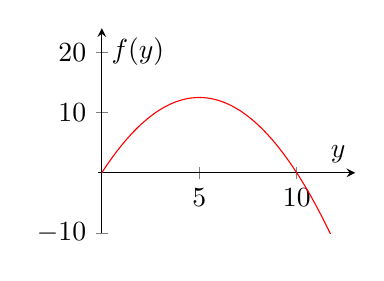
\begin{tikzpicture}
            \begin{axis}[width=0.4\textwidth, axis lines=middle, xlabel=$y$, ylabel=$f(y)$, xmin=-.2, ymin=-10, ymax=24, xmax=13]
                \addplot[color=red,domain=0:20,samples=200]{5 * x - 0.5 * x * x};
            \end{axis}
        \end{tikzpicture}
    \end{figure}
Here, $K = 10$, so we have critical points at $y=0$ and $y=10=K$. Because we have $\dv{y}{t} = f(y)$, the direction that $y$ moves can be thought of as being represented by the sign of $f$. For $0 < y < K$, we have $f(y) > 0$, which means that as time progresses, $y$ will increase. This means that if we place some initial point $(y, f(y))$ on the interval $y \in [0, K]$, the point will naturally want to move right along the graph until it reaches $(K, f(K)) = (K, 0)$, where it will stop. Similarly, for $y > K$, we have $f(y) < 0$. So any point placed on the interval $y\in [K, \infty)$ will naturally ant to move left along the graph until it reaches $(K,0)$. \par
We can also pay attention to the relationship between this graph and the steepness of our solution. Because $\dd y/\dd t = f(y)$, the steepness of the graph of a solution curve at some $y=y_0$ is $\abs{\dv{y}{t} \,(y_0)} = \abs{f(y_0)}$. Graphically, this is the distance between the $y$ axis and the height of $f(y)$. This tells us that points near $y=0$ and $y=K$ will have relatively flat solution curves, and points near the middle, around $y=K/2$ (as well as points with $y \gg K$), will have very steep solution curves. \par
More meaning can be gleamed from this geometric model by analyzing the concavity of $y$. We can use the chain rule to say
\[ \dv[2]{y}{t} = \dv{t} \dv{y}{t} = \dv{t} f(y) = \dv{f}{y}\dv{y}{t} = f'(y)f(y) \]
The graph of $y$ versus $t$ will be concave up when $f'(y)$ and $f(y)$ agree in sign. This will occur when the graph of $f(y)$ versus $y$ is positive and increasing or negative and decreasing. Similarly, the graph of $y$ versus $t$ is concave down when $f'(y)$ and $f(y)$ have opposite signs--when the graph of $f(y)$ versus $y$ is positive and decreasing or negative and increasing. Inflection points will occur when $f'(y)$ \it{or} $f(y)$ are zero. \par
Applying this to the above graph, we can see that $y(t)$ is concave up on the interval $(0, K/2)$, concave down on the interval $(K/2, K)$, and concave up on the interval $(K, \infty)$. Inflection points occur at the equilibrium points and at the vertex of the parabola: when $y=0,K/2$ or $K$. \par
Notice that we were able to make many qualitative observations about the behavior of the differential equation without ever needing to solve it explicitly. In many cases, these qualitative facts are more than enough to derive sufficient understanding of the situation. 
\end{example}
\begin{example}
    Now, consider the differential equation
    \[ \dv{y}{t} = -ry \pqty{1-\frac{y}{T}} \]
    where $r,T\in\RR_+$. Despite the fact that this differs from the logistic differential equation by only a factor of $-1$, the behavior of the solutions will differ greatly. \par
    Equilibrium solutions are located at $y=0$ and $y=T$, and the graph of $f(y)$ versus $y$ looks like this (with $T=10$):
    \begin{figure}[h!]
        \centering
        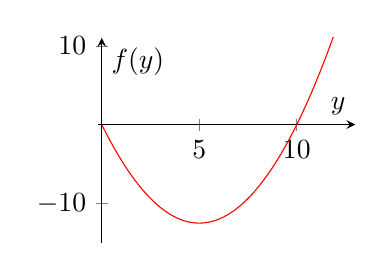
\begin{tikzpicture}
            \begin{axis}[width=0.4\textwidth, axis lines=middle, xlabel=$y$, ylabel=$f(y)$, xmin=-.2, ymin=-15, ymax=11, xmax=13]
                \addplot[color=red,domain=0:20,samples=200]{- 5 * x + 0.5 * x * x};
            \end{axis}
        \end{tikzpicture}
    \end{figure}
    With all solutions starting on the interval $0 < y < T$ approaching $y=0$ and solutions on the interval $y > T$ diverging towards infinity. Thus $y=0$ is a stable equilibrium point and $y=T$ is an unstable equilibrium point. \par
    Further, points above $y=T$ cause $y(t)$ to be concave up, so it will increase without bound at an increasing rate. \par
    Notice that all solutions below or equal to $T$ will eventually approach a finite, constant value, while solutions above $T$ will diverge towards infinity. In cases like this, we call $T$ a \bf{threshold level} for the differential equation. \par
    Through separation of variables, we can come up with an equation that solves this differential equation subject to the initial condition $y(0) = y_0$:
    \[ y(t) = \frac{y_0T}{y_0 + (T-y_0)e^{rt}} \]
    If $0 < y_0 < T$, then we can notice that as $t\to\infty$, the denominator grows extremely quickly and $y(t)$ approaches $0$. \par
    If $y_0 > T$, then we will have the denominator approaching a large negative value, causing the solution to also approach zero. However, there will be a vertical asymptote when the denominator changes sign from positive to negative. Specifically, the asymptote occurs at the $t$ value $t^*$ such that $y_0 + (T-y_0)e^{rt^*} = 0$, or
    \[ t^* = \frac{1}{r}\ln \frac{y_0}{y_0-T}\]
    Notice that this asymptotic behavior could not have been predicted by our qualitative analysis of the behavior of the equation. This is one scenario where attempting to find a concrete numerical solution will bring us extra information we could not otherwise find. 
\end{example}
\subsection{Exact Differential Equations and Integrating Factors}
Here, we explore another family of differential equations that we are able to solve. 
\begin{example}
    Solve the differential equation
    \[ 2x + y^2 + 2xy\dv{y}{x} = 0 \] 
    \bf{Solution:} This equation is neither linear nor separable, so we cannot apply any of those methods. However, take notice that for a function $\psi(x, y) = x^2+xy^2$, we have
    \[ \pdv{\psi}{x} = 2x + y^2 \quad\text{and}\quad \pdv{\psi}{y} = 2xy \]
    This allows us to rewrite the differential equation as
    \[ \pdv{\psi}{x} + \pdv{\psi}{y}\dv{y}{x} = 0\]
    Which we can recognize as the multivariable chain rule applied to $\dv{x} \psi(x,y(x))$. Therefore, we can rewrite to obtain
    \[ \dv{\psi}{x} = 0 \]
    or
    \[ \psi(x,y) = x^2 + xy^2 = C \]
    Which implicitly defines our general solution.
\end{example}
In the previous example, the key step was the ability to recognize the magic function $\psi$ that allows us to rewrite the equation. More generally, for the differential equation
\[ M(t,x ) + N(t, x)\dv{x}{t} = 0\]
We seek to find some function $\psi(t, x)$ such that
\[ \pdv{\psi}{t} = M(t, x) \quad \text{and}\quad \pdv{\psi}{x} = N(t,x)\]
Equations of this form are known as \bf{exact differential equations} because they can be expressed exactly as the derivative of some function, and are implicitly solved by 
\[ \psi(t, x) = C\]
where $C$ is an arbitrary constant. \par
But how can we know if a differential equation is exact? The previous example was relatively easy to identify, but what if that is not the case in the future? \par
To analyze this, let's take a look at what it means for an equation to be exact. First, we can notice that the vector $\< \partial \psi /\partial x, \partial \psi/\partial t\>$ is precisely equal to $\grad \psi$. Therefore, the claim that some $\psi$ exists such that $\grad\psi = \< M(t,x), N(t,x)\>$ is equivalent to saying that the field $\< M(t,x), N(t,x)\>$ is conservative. \par
Therefore, we can guarantee that a differential equation is exact if 
\[ \pdv{M}{x} - \pdv{N}{t} = 0\]
As for how to find the function $\psi$, it is the same process as finding the potential function for a vector field. It may prove useful to brush up on your Calculus III skills if you forgot how to do this. 
\begin{example}
    Solve the differential equation
    \[ (y\cos x + 2xe^y) + (\sin x + x^2e^y-1)\dv{y}{x} = 0 \]
    \bf{Solution:} First, we can verify that this is an exact differential equation:
    \[ \pdv{y} (y\cos x + 2xe^y) = \cos x + 2xe^y \]
    \[ \pdv{x} (\sin x + x^2e^y - 1) = \cos x + 2xe^y \]
    These are equal, so the equation is exact. Our function $\psi(x,y)$ is the function that satisfies
    \begin{align*}
        \pdv{\psi}{x} &= y\cos x + 2xe^y \\
        \pdv{\psi}{y} &= \sin x + x^2e^y - 1
    \end{align*} 
    Integrating both of these equations, we find
    \begin{align*}
        \psi(x,y) &= y\sin x + x^2e^y + C_1(y) \\
        \psi(x,y) &= y\sin x + x^2e^y - y + C_2(x)
    \end{align*}
    Which can be combined to give us
    \[ \psi(x,y) = y\sin x + x^2e^y - y \]
    We do not include a $+C$ because we already have one in the next step. \par
    Now, we obtain $\dd \psi / \dd x = 0$, which implicitly defines our solution as
    \[ y\sin x + x^2e^y - y = C \]
\end{example}
\subsubsection{Integrating Factors}
It is sometimes possible to convert a differential equation that is not exact into an exact differential equation by multiply the equation by a suitable integrating factor. Suppose the have a differential equation given by 
\[ M(x,y) + N(x,y)\dv{y}{x} = 0 \]
Multiply the equation by a nonzero function $\mu(x,y)$ chosen so that the following equation is exact.
\[ \mu(x,y)M(x,y) + \mu(x,y)N(x,y)\dv{y}{x} \]
That is, we choose our $\mu$ so that 
\[ \pdv{y} \pqty{\mu M} = \pdv{x} \pqty{\mu N} \]
By the product rule, we can rewrite this equation as
\[ \pdv{\mu}{y}M + \mu \pdv{M}{y} = \pdv{\mu}{x}N + \mu\pdv{N}{x} \]
Or,
\begin{equation} \label{intfacteq}
    M\pdv{\mu}{y} - N\pdv{\mu}{x} + \bqty{\pdv{M}{y} - \pdv{N}{x}}\mu = 0
\end{equation}
There may be multiple solutions to this partial differential equation, in which case any solution is applicable. \par
While the idea of an integrating factor is in theory helpful in a broad number of situations, its usefulness is limited because it can be extremely difficult to determine what function to pick for $\mu$. Solving equation \ref{intfacteq} is often just as hard as solving the original differential equation. \par
We will limit our search to a special case that allows us to more easily find a suitable $\mu$. \par 
If $\mu$ is a pure function of $x$ or $y$ (rather than a function of both), one of the partials of $\mu$ will reduce to zero and the other will become a total derivative. For demonstration, let $\mu$ be a pure function of $x$. Then, Equation \ref{intfacteq} becomes
\[ -N\dv{\mu}{x} + \bqty{\pdv{M}{y} - \pdv{N}{x}}\mu = 0\]
which gives us a first order differential equation for $\mu$:
\[ \dv{\mu}{x} = \frac{1}{N} \bqty{\pdv{M}{y} - \pdv{N}{x}}\mu \]
As long as $N\neq 0$.\par 
Using the more concise notation $\partial M/\partial y = M_y$, we can write
\[ \dv{\mu}{x} = \frac{M_y-N_x}{N}\mu \]
If $(M_y-N_x)/N$ depends solely on $x$, then $\mu$ is a pure function of $x$ which allows us to solve for it using the method of separation of variables. \par
A similar procedure can occur for when $(M_y-N_x)/N$ is solely dependent on $y$.
\begin{example}
    Find an integrating factor for the equation 
    \[ \pqty{3xy + y^2} + \pqty{x^2+xy}\dv{y}{x} = 0 \]
    and then solve the equation. \par
    \bf{Solution:} First, we can verify that the equation is not already exact.
    \begin{align*}
        \pdv{y} \pqty{3xy + y^2}  &= 3x + 2y \\
        \pdv{x} \pqty{x^2+xy} &= 2x +y 
    \end{align*}
    These are not equal, so the equation is not already exact. Now, we can attempt to find an integrating factor by computing $(M_y-N_x)/N$.
    \begin{align*}
        \frac{M_y - N_x}{N} &= \frac{(3x+2y)-(2x+y)}{x^2+xy} \\
        &= \frac{x+y}{x(x+y)} = \frac{1}{x}
    \end{align*}
    This is a sole function of $x$, so the integrating factor $\mu(x)$ will also be a sole function of $x$, as desired. \par
    The differential equation for $\mu(x)$ is given by
    \[ \dv{\mu}{x} = \frac{1}{x} \mu \]
    Which is solved with $\mu(x) = x$. Multiplying the original differential equation by this integrating factor, we find
    \[ (3x^2y+xy^2) + (x^3+x^2y)\dv{y}{x} = 0 \]
    We can check that this new equation is exact:
    \begin{align*}
        \pdv{y} \pqty{3x^2y + xy^2}  &= 3x^2 + 2xy \\
        \pdv{x} \pqty{x^3+x^2y} &= 3x^2+2xy
    \end{align*}
    These are equal, so the equation is exact. Now, we can find $\psi(x,y)$.
    \begin{align*}
        \psi(x,y) &= \int (3x^2y+xy^2)\dd x = x^3y + \frac{1}{2}x^2y^2 + C_1(y) \\
        \psi(x,y) &= \int (x^3 + x^2y)\dd y = x^3y + \frac{1}{2}x^2y^2+ C_2(x)
    \end{align*}
    Which can be combined to give us $\psi = x^3y + \frac{1}{2}x^2y^2$. This gives us the implicit solution
    \[ x^3y + \frac{1}{2}x^2y^2 = C \]
\end{example}
\subsection{First Order Difference Equations}
So far we have focused our explanation on ways of modeling continuous situations with differential equations. However, there are cases where a discrete model proves more useful or natural. For example, the interest in bank accounts is far more often done in discrete intervals rather than following a continuous function. \par
In general, a \bf{first order difference equation} is an equation of the form
\[ y_{n+1} = f(n, y_n), \quad\quad n\in\NN \]
Sometimes accompanied by an initial condition $y_0 = \alpha$. \par
In the special case where $f$ does not depend on $n$, so
\[ y_{n+1} = f(y_n) \]
We can find $y_n$ for any $n$ with repeated applications of $f$. We have
\[ y_1 = f(y_0) \quad y_2 = f(f(y_0)) \]
and this pattern will repeat until we find
\[ y_n = \underset{\text{(n times)}}{f(f(\cdots }(y_0))) \]
We denote this as $y_n = f^n(y_0)$. Repeatedly applying $f$ is known as \bf{iterating} the difference equation and is of particular interest when attempting to analyze the limit of the sequence. \par
Solutions for which every $y_n$ has the same value are called \bf{equilibrium soutions}, and are found by solving the equation
\[ y_n = f(y_n) \]
for $y_n$.
\subsubsection{First Order Linear Difference Equations}
A first order difference equation is linear if it can be written in the form
\[ y_{n+1} = \rho_ny_n, \quad\quad n\in\NN\]
By iteration, this lets us obtain
\[ y_n = \rho_{n-1}\cdots\rho_1\rho_0 y_0 \]
One useful fact that this equation tells us is that if $\rho_n$ is zero for some $n$, then all successive values of $y_N$, $N\geq n$ are also zero. \par
If the constant $\rho_n$ has the same value $\rho$ for every $n$, then the difference equation becomes
\[ y_{n+1} = \rho y_n\]
and it is solved by $y_n = \rho^n y_0$. For this difference equation, the limiting behavior is quite easy to find:
\[ \lim_{n\to\infty} y_n = \lim_{n\to\infty}\rho^n y_0 = \begin{cases}
    0, & \abs{\rho} < 1 \\
    y_0 & \rho = 1 \\
    \text{does not exist} & \text{otherwise}
\end{cases}\]
So the equilibrium solution $y = y_0$ for $\rho = 1$ is unstable, and the equilibrium solution $ y = 0$ is stable for $\abs{\rho} < 1$ and unstable for $\abs{\rho} > 1$. \par
Now, consider a model where
\[ y_{n+1} = \rho y_n + b_n, \quad \quad b\in\NN\]
We can solve this by iteration, just as we did before. 
\begin{align*}
    y_1 &= \rho y_0 + b_0 \\
    y_2 &= \rho (\rho y_0 + b_0) + b_1 = \rho^2 y_0 + \rho b_0 + b_1 \\
    y_3 &= \rho^3 y_0 + \rho^2 b_0 + \rho b_1 + b_2
\end{align*}
And so on until we find
\[ y_n = \rho^n y_0 + \sum_{i=0}^n \rho^{n-i-1}b_i \]
If we have each $b_n$ equal to a constant $b$, then we instead find
\[ y_n = \rho^n y_0 + (1 + \rho + \rho^2 + \cdots + \rho^{n-1})b\]
From the formula for the sum of a finite geometric series, we can say (for $\rho \neq 1$) that
\[ y_n = \rho^n y_0 + \frac{1-\rho^n}{1-\rho}b\]
We can rewrite this one last time to make the behavior of this solution more clear.
\[ y_n = \rho^n \pqty{y_0 - \frac{b}{1-\rho}} + \frac{b}{1-\rho} \]
If $\abs{\rho} < 1$, then the $\rho^n$ term goes to zero and the sequence converges to $b/(1-\rho)$. If $\abs{\rho} > 1$ or $\rho = -1$, then the sequence does not converge. \par 
If $\rho = 1$, then the formula itself is not valid (due to the $1-\rho$ in the denominators), and we have to return to the original difference equation:
\[ y_n = \rho^n y_0 + (1 + \rho + \cdots + \rho^{n-1})b = y_0 + bn\]
Which grows without bound as $n\to\infty$.